\begin{table}[h!]
    \caption{Resultados da calibração das leituras de \acrshort{no2} do sensor NO2-B43F}
    \centering
    \begin{tabularx}{0.95\textwidth}[h!]{
        >{\raggedright\hsize=.4\hsize\arraybackslash}X
        >{\raggedright\hsize=.6\hsize\arraybackslash}X 
        >{\raggedright\hsize=.6\hsize\arraybackslash}X
        >{\raggedright\hsize=.7\hsize\arraybackslash}X 
        >{\raggedright\hsize=.6\hsize\arraybackslash}X 
        >{\raggedright\hsize=.3\hsize\arraybackslash}X }
        \hline
        Var. & Modelo & R2 & RMSE & MAE & $\rho$\\ [0.5ex]
        \hline
        \acrshort{no2} & \textbf{MLP}: & -3.95 ± 5.68 & -12.87 ± 3.90 & -9.94 ± 2.52 & -- \\ [0.5ex]
           & \textbf{MLR} & -3.80 ± 6.39 & -12.61 ± 3.74 & -9.62 ± 2.17 & -- \\ [0.5ex]
           & \textbf{KNN:} & -3.73 ± 5.49 & -12.84 ± 3.67 & -9.92 ± 2.10 & -- \\ [0.5ex]
           & \textbf{RF:} & -4.39 ± 6.07 & -13.70 ± 3.50 & -10.33 ± 2.08 & -- \\ [0.5ex]
        \hline
        \acrshort{no2}, T & \textbf{MLP:} & -2.84 ± 4.36 & -11.76 ± 3.40 & -9.00 ± 1.81 & 0.59 \\ [0.5ex]
              & \textbf{MLR:} & -3.62 ± 5.88 & -12.57 ± 3.40 & -9.70 ± 1.87 & -- \\ [0.5ex]
              & \textbf{KNN:} & -2.62 ± 4.52 & -12.02 ± 3.33 & -8.88 ± 1.54 & 0.61 \\ [0.5ex]
              & \textbf{RF:} & -2.66 ± 4.51 & -11.93 ± 3.39 & -9.18 ± 2.03 & 0.63 \\ [0.5ex]
        \hline
    \end{tabularx}
    \label{tab:data-no2-calib-results}
\end{table}

% ----------------------------------------------------------
\section{Correção das leituras do sensor NO2-B43F com as medições de referência}
% ----------------------------------------------------------

A partir dos dados de referência e das leituras de concentração e temperatura adquiridas pelo monitor em questão, foi realizada uma busca em grid para encontrar as melhores combinações de parâmetros e variáveis de entrada a modelos de regressão. As variáveis que foram testadas como entrada foram as leituras de concentração de \acrshort{no2} do sensor NO2-B43F e a temperatura no interior da câmara de medição. Como modelos de regressão foram testados: o Perceptron Multicamadas (MLP), a Regressão Linear Multivariada (MLR), os K Vizinhos mais Próximos (KNN) e as Florestas Aleatórias (RF). Na Tabela \ref{tab:data-no2-calib-results} resumem-se os melhores modelos encontrados pela busca em \textit{grid} para calibrar as leituras do sensor de baixo custo. Os mesmos resultados são ilustrados graficamente na Figura \ref{fig:data-no2-models-performance} que apresenta o desempenho dos modelos e as variáveis de entrada considerando os valores de R2, RMSE e MAE.

\begin{figure}[h!]
    \centering
    \caption{Resultados dos modelos de calibração aplicados as leituras de \acrshort{no2} do sensor NO2-B43F}
    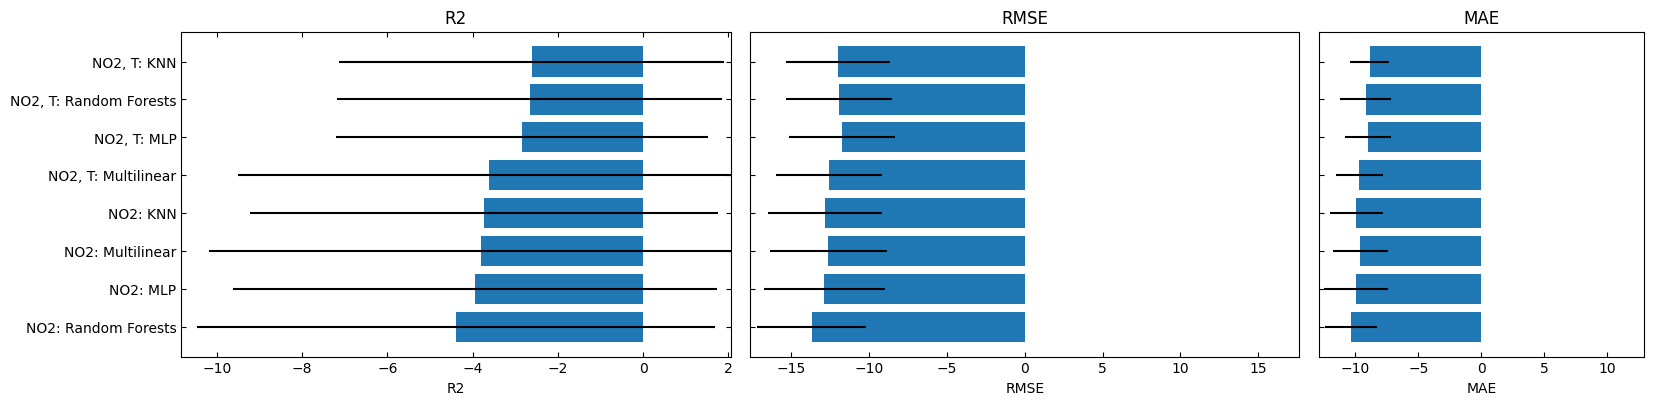
\includegraphics[width=0.95\textwidth]{chapters/4-CALIBRAÇÃO MÚLTIPLOS SENSORES/Figuras/no2-B43F-models-performance.png}
    \label{fig:data-no2-models-performance}
\end{figure}

\begin{figure}[h!]
    \centering
    \caption{Gráfico de dispersão das leituras do sensor de \acrshort{no2} NO2-B43F e a estação de referência após aplicar modelos de regressão considerando a temperatura}
    \begin{subfigure}{0.49\textwidth}
        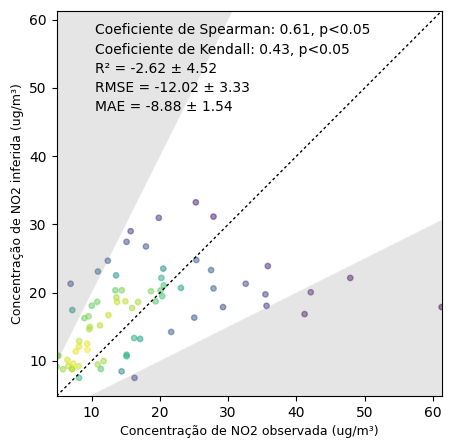
\includegraphics[width=\textwidth]{chapters/4-CALIBRAÇÃO MÚLTIPLOS SENSORES/Figuras/no2-T-KNN-Regression.png}
        \caption{Utilizando uma regressão pelos k vizinhos mais próximos considerando a temperatura obteve-se um $\rho$ de 0.61}
        \label{fig:data-no2-T-reference-corr-KNN}
    \end{subfigure}
    \hfill
    \begin{subfigure}{0.49\textwidth}
        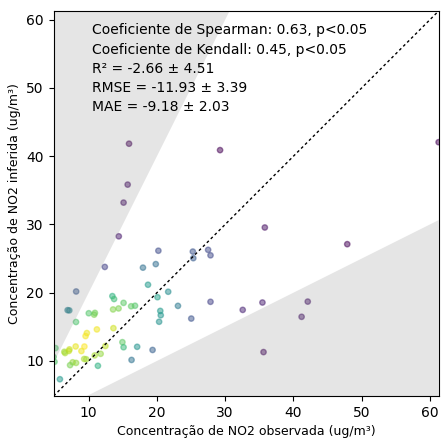
\includegraphics[width=\textwidth]{chapters/4-CALIBRAÇÃO MÚLTIPLOS SENSORES/Figuras/no2-T-RF-Regression.png}
        \caption{Utilizando uma regressão por Florestas Aleatórias considerando a temperatura obteve-se um valor de $\rho$ de 0.63}
        \label{fig:data-no2-T-reference-corr-RF}
    \end{subfigure}
\end{figure}

Como se observa todas as variantes de modelos e variáveis de entrada apresentaram valores de R2 negativos, indicando que nenhum dos modelos foi capaz de explicar a variância na variável dependente, i.e. a concentração real. Observa-se também que nenhum dos modelos uni-variados conseguiu que os dados observados e os inferidos apresentassem alguma correlação. Por outro lado, os modelos multivariados, a exceção da regressão linear, que incluíram a temperatura como variável de entrada, produziram coeficientes de correlação entre a concentração real e a medida pelo sensor, entre 0.59 - 0.63. As Figuras \ref{fig:data-no2-T-reference-corr-KNN} e \ref{fig:data-no2-T-reference-corr-RF} apresentam os resultados ao aplicar os modelos de k Vizinhos mais Próximos e Florestas Aleatórias.

\begin{figure}[h!]
    \centering
    \caption{Desempenho dos modelos de regressão aplicados para inferir as leituras de concentração de \acrshort{no2} medidas pela estação de referência}
    \begin{subfigure}{0.9\textwidth}
        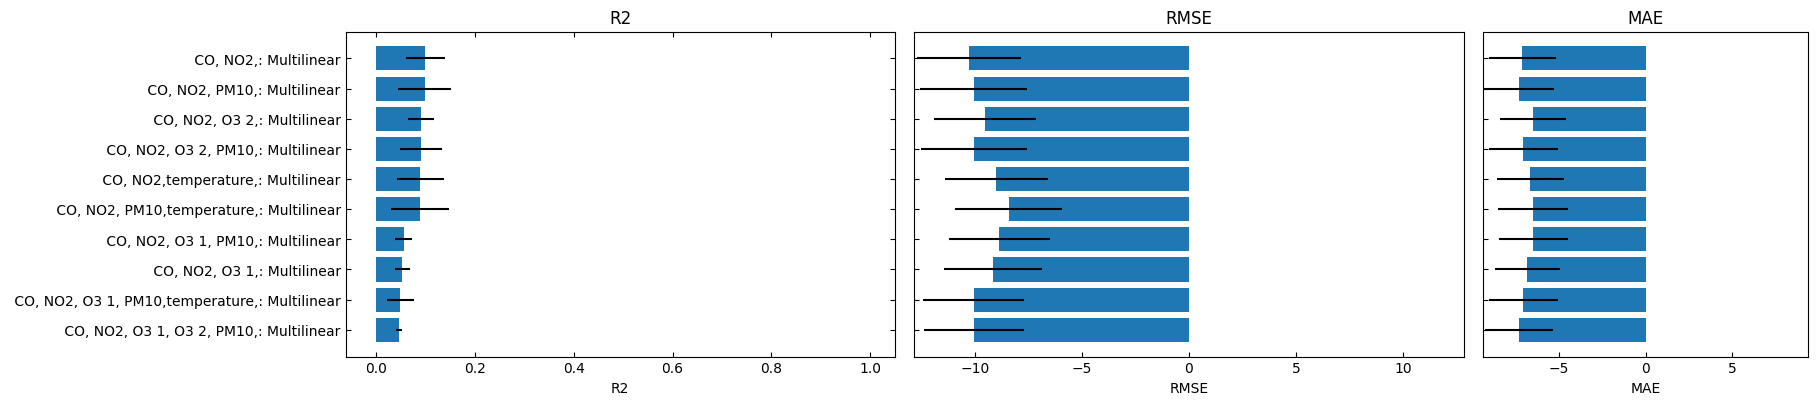
\includegraphics[width=\textwidth]{chapters/4-CALIBRAÇÃO MÚLTIPLOS SENSORES/Figuras/no2-all-models-performance.png}
        \caption{Valores de R2, RMSE e MAE obtidos pelos 10 modelos com maiores valores de R2}
        \label{fig:data-no2-all-models-performance}
    \end{subfigure}
    \begin{subfigure}{0.9\textwidth}
        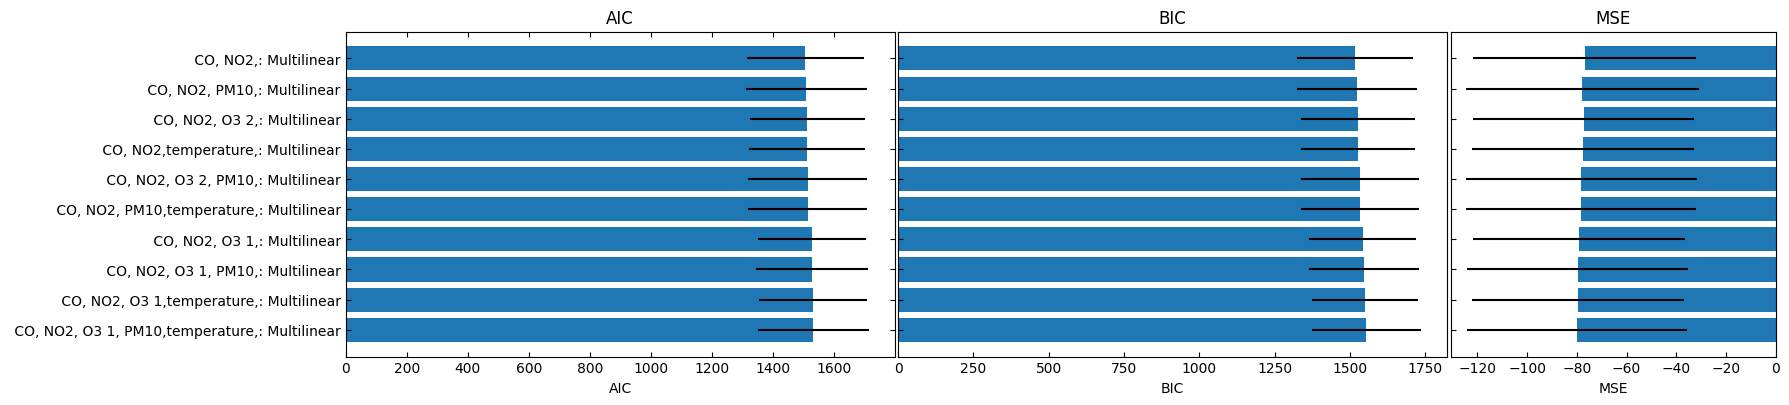
\includegraphics[width=\textwidth]{chapters/4-CALIBRAÇÃO MÚLTIPLOS SENSORES/Figuras/no2-all-models-complexity.png}
        \caption{Modelos com menores valores de \acrshort{aic} e \acrshort{bic}}
        \label{fig:data-no2-all-models-comlexity}
    \end{subfigure}
    \label{fig:data-no2-all-models-performance-comlexity}
\end{figure}

\begin{figure}[h]
    \centering
    \caption{Gráfico de dispersão das leituras de múltiplos sensores e a estação de referência para medição de \acrshort{no2}}
    \begin{subfigure}{0.49\textwidth}
        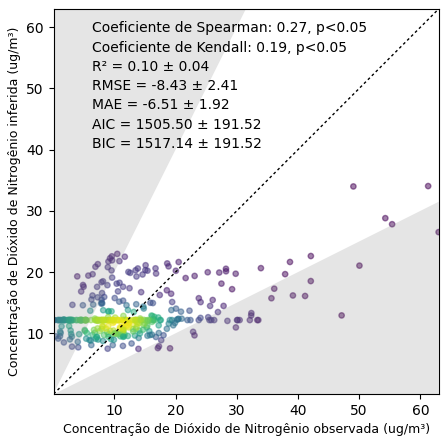
\includegraphics[width=\textwidth]{chapters/4-CALIBRAÇÃO MÚLTIPLOS SENSORES/Figuras/NO2-co-no2-Multilinear-Regression.png}
        \caption{Utilizando modelo de regressão linear multivariado com variáveis independentes: leituras de sensores CO-B4, e NO2-B43F}
        \label{fig:data-co-no2-reference-NO2-corr-MLR}
    \end{subfigure}
    \hfill
    \begin{subfigure}{0.49\textwidth}
        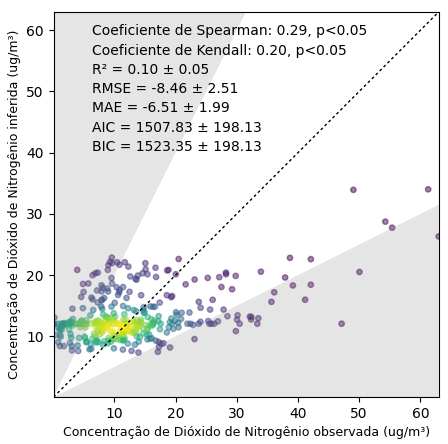
\includegraphics[width=\textwidth]{chapters/4-CALIBRAÇÃO MÚLTIPLOS SENSORES/Figuras/NO2-co-no2-pm10-Multilinear-Regression.png}
        \caption{Utilizando modelo de regressão linear multivariado com variáveis independentes: leituras de sensores CO-B4, NO2-B43F e sensor de \acrshort{mp10} OPC-N3}
        \label{fig:data-co-no2-pm10-reference-NO2-corr-RF}
    \end{subfigure}
\end{figure}

% ----------------------------------------------------------
\section{Cálculo da concentração de Dióxido de Nitrogênio a partir das leituras do arranjo de sensores de gases}
% ----------------------------------------------------------

A Figura \ref{fig:data-no2-all-models-performance} apresenta os valores de R2 dos 10 melhores modelos de calibração calculados para as leituras de \acrshort{no2}. Observa-se que os valores de R2 desses 10 modelos apresentaram valores de R2 em média positivos, com valores máximos de até aproximadamente 0.2, todos obtidos a partir de regressões lineares. Com relação as variáveis de entrada observa-se que todos os 10 modelos consideraram o \acrshort{co} com variações nos restantes das variáveis para cada modelo. Com relação à complexidade dos modelos (Figura \ref{fig:data-no2-all-models-performance-comlexity}) observa-se que o ranqueamento por \acrshort{aic} coincidiu bastante com o ranqueamento por R2. As Figuras \ref{fig:data-co-no2-reference-NO2-corr-MLR} e \ref{fig:data-co-no2-pm10-reference-NO2-corr-RF} mostram os resultados obtidos com os dois modelos com maior R2 médio, i.e.: regressões lineares com variáveis de entrada leituras de sensores CO-B4 e NO2B43F, e leituras de sensores CO-B4, NO2B43F e sensor de \acrshort{mp10} OPC-N3, respectivamente. As figuras mostram gráficos de dispersão entre os dados calibrados por esses modelos e as leituras de referência.